\chapter{Heritage}
\label{chap:heritage}
\graphicspath{{Mission_Heritage/Images/}}

In the past, there have been multiple spacecraft missions to the small bodies in our Solar System which have collectively increased our understanding about them. While a large majority of these have been asteroid fly-by scenarios, a few have also been rendezvous missions \parencite{esa_mission2asteroids_web}. This chapter will provide an overview on few of these missions followed by a brief literature review which shall be of interest to the thesis at hand. This will help us in justifying the research objectives mentioned in \Cref{chap:research_questions}. \Cref{sec:past_missions} will discuss the asteroid rendezvous missions which have already taken place, \Cref{sec:future_missions} will discuss future rendezvous missions, and finally, \Cref{sec:literature_review} will discuss the state-of-the-art.

\section{Past Missions}
\label{sec:past_missions}
In all the history of space exploration there have been only three spacecraft missions that have rendezvoused with asteroids. In chronological order these are: \gls{NASA}'s \gls{NEAR}-Shoemaker mission to asteroid Eros, \gls{JAXA}'s Hayabusa mission to asteroid Itokawa, and \gls{NASA}'s Dawn mission to asteroids Vesta and Ceres.

\subsection{NEAR-Shoemaker}
\label{subsec:near_heritage}
The \gls{NEAR}-Shoemaker (henceforth \gls{NEAR}) mission was launched in 1996 and rendezvoused with Eros in 2000. Its operational phase around the asteroid continued for about a year during which it obtained several high-resolution images of the surface and collected comprehensive measurements to estimate its internal mass distribution, shape model, gravity and spin state amongst other observations \parencite{scheeresBook}. The bulk density of Eros was estimated to be $2.67 \pm 0.03 [g/cm^3]$ and its mass to be $(6.6904 \pm 0.003) \times 10^{15} [kg]$. The rotation state was estimated to be $1639.38922 \pm 0.00015$ [deg/day] which gives a rotational period of about $5.27$ [hrs] \parencite{erosShapeDetermination}. On 25 October 2000, \gls{NEAR} executed a \gls{LAF} over Eros in which it acquired several high-resolution images that helped in understanding the surface morphology. The images confirmed the existence of a substantial amount of regolith on the surface with a typical thickness value of tens of metres over the bedrock, except of course on steep slopes. The regolith was found to be highly complex, in that it varied from fine material to metre-sized ejecta blocks \parencite{Veverka2001}. \cite{Robinson2001} estimates the size of the finer regolith to be around 1.0 [cm] or smaller from images that had a resolution of 1.2 [cm] per pixel. \Cref{fig:eros_regolith} depicts the regolith morphology in one of the high-resolution imaging sequences from the \gls{LAF} \parencite{veverka2001landing}.
%%%
\begin{figure}[htb]
\centering
\captionsetup{justification=centering}
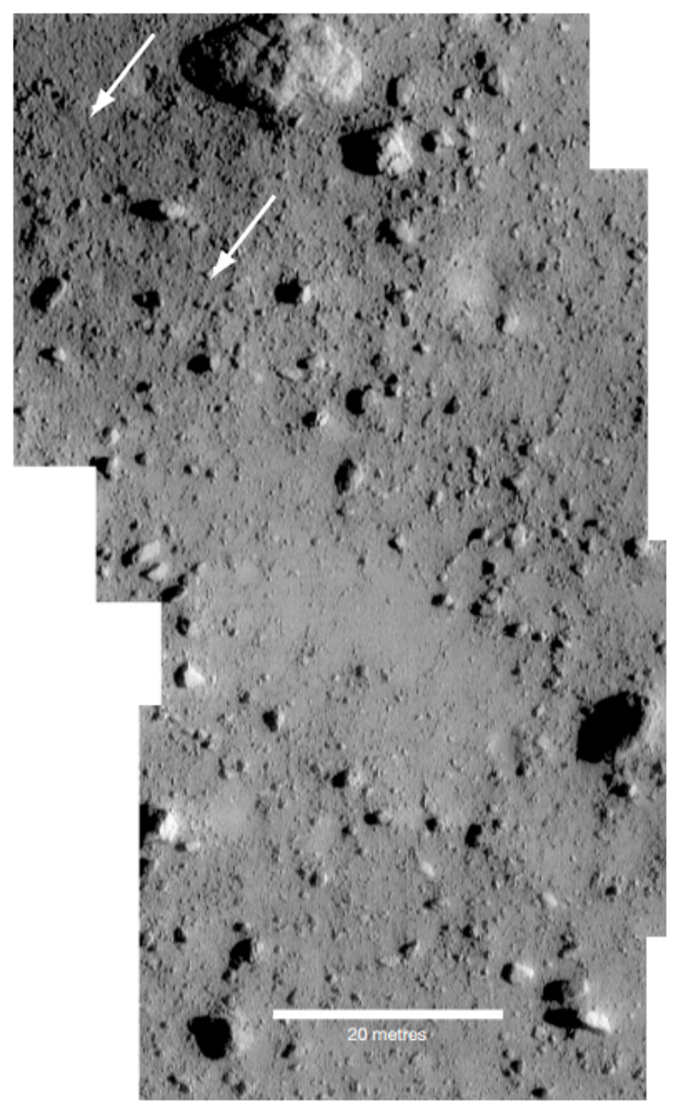
\includegraphics[width=\linewidth, height=0.5\textheight, keepaspectratio=true]{eros_regolith.pdf}
\caption{Mosaic of high-resolution images depicting the nature of regolith on the surface of Eros \parencite{veverka2001landing}.}
\label{fig:eros_regolith}
\end{figure}
\FloatBarrier
%%%

\section{Future Missions}
\label{sec:future_missions}


\section{State of the art / Literature Review}
\label{sec:literature_review}
